\documentclass[twoside]{book}

% Packages required by doxygen
\usepackage{fixltx2e}
\usepackage{calc}
\usepackage{doxygen}
\usepackage[export]{adjustbox} % also loads graphicx
\usepackage{graphicx}
\usepackage[utf8]{inputenc}
\usepackage{makeidx}
\usepackage{multicol}
\usepackage{multirow}
\PassOptionsToPackage{warn}{textcomp}
\usepackage{textcomp}
\usepackage[nointegrals]{wasysym}
\usepackage[table]{xcolor}

% Font selection
\usepackage[T1]{fontenc}
\usepackage[scaled=.90]{helvet}
\usepackage{courier}
\usepackage{amssymb}
\usepackage{sectsty}
\renewcommand{\familydefault}{\sfdefault}
\allsectionsfont{%
  \fontseries{bc}\selectfont%
  \color{darkgray}%
}
\renewcommand{\DoxyLabelFont}{%
  \fontseries{bc}\selectfont%
  \color{darkgray}%
}
\newcommand{\+}{\discretionary{\mbox{\scriptsize$\hookleftarrow$}}{}{}}

% Page & text layout
\usepackage{geometry}
\geometry{%
  a4paper,%
  top=2.5cm,%
  bottom=2.5cm,%
  left=2.5cm,%
  right=2.5cm%
}
\tolerance=750
\hfuzz=15pt
\hbadness=750
\setlength{\emergencystretch}{15pt}
\setlength{\parindent}{0cm}
\setlength{\parskip}{3ex plus 2ex minus 2ex}
\makeatletter
\renewcommand{\paragraph}{%
  \@startsection{paragraph}{4}{0ex}{-1.0ex}{1.0ex}{%
    \normalfont\normalsize\bfseries\SS@parafont%
  }%
}
\renewcommand{\subparagraph}{%
  \@startsection{subparagraph}{5}{0ex}{-1.0ex}{1.0ex}{%
    \normalfont\normalsize\bfseries\SS@subparafont%
  }%
}
\makeatother

% Headers & footers
\usepackage{fancyhdr}
\pagestyle{fancyplain}
\fancyhead[LE]{\fancyplain{}{\bfseries\thepage}}
\fancyhead[CE]{\fancyplain{}{}}
\fancyhead[RE]{\fancyplain{}{\bfseries\leftmark}}
\fancyhead[LO]{\fancyplain{}{\bfseries\rightmark}}
\fancyhead[CO]{\fancyplain{}{}}
\fancyhead[RO]{\fancyplain{}{\bfseries\thepage}}
\fancyfoot[LE]{\fancyplain{}{}}
\fancyfoot[CE]{\fancyplain{}{}}
\fancyfoot[RE]{\fancyplain{}{\bfseries\scriptsize Generated by Doxygen }}
\fancyfoot[LO]{\fancyplain{}{\bfseries\scriptsize Generated by Doxygen }}
\fancyfoot[CO]{\fancyplain{}{}}
\fancyfoot[RO]{\fancyplain{}{}}
\renewcommand{\footrulewidth}{0.4pt}
\renewcommand{\chaptermark}[1]{%
  \markboth{#1}{}%
}
\renewcommand{\sectionmark}[1]{%
  \markright{\thesection\ #1}%
}

% Indices & bibliography
\usepackage{natbib}
\usepackage[titles]{tocloft}
\setcounter{tocdepth}{3}
\setcounter{secnumdepth}{5}
\makeindex

% Hyperlinks (required, but should be loaded last)
\usepackage{ifpdf}
\ifpdf
  \usepackage[pdftex,pagebackref=true]{hyperref}
\else
  \usepackage[ps2pdf,pagebackref=true]{hyperref}
\fi
\hypersetup{%
  colorlinks=true,%
  linkcolor=blue,%
  citecolor=blue,%
  unicode%
}

% Custom commands
\newcommand{\clearemptydoublepage}{%
  \newpage{\pagestyle{empty}\cleardoublepage}%
}

\usepackage{caption}
\captionsetup{labelsep=space,justification=centering,font={bf},singlelinecheck=off,skip=4pt,position=top}

%===== C O N T E N T S =====

\begin{document}

% Titlepage & ToC
\hypersetup{pageanchor=false,
             bookmarksnumbered=true,
             pdfencoding=unicode
            }
\pagenumbering{alph}
\begin{titlepage}
\vspace*{7cm}
\begin{center}%
{\Large Week 10 Assignment \\[1ex]\large 1.\+0 }\\
\vspace*{1cm}
{\large Generated by Doxygen 1.8.13}\\
\end{center}
\end{titlepage}
\clearemptydoublepage
\pagenumbering{roman}
\tableofcontents
\clearemptydoublepage
\pagenumbering{arabic}
\hypersetup{pageanchor=true}

%--- Begin generated contents ---
\chapter{File Index}
\section{File List}
Here is a list of all documented files with brief descriptions\+:\begin{DoxyCompactList}
\item\contentsline{section}{/home/markose/catkin\+\_\+ws/src/begineer\+\_\+tutorials/src/\hyperlink{listener_8cpp}{listener.\+cpp} \\*Subscriber for beginner tutorials  M\+IT License 2021 Markose Jacob }{\pageref{listener_8cpp}}{}
\item\contentsline{section}{/home/markose/catkin\+\_\+ws/src/begineer\+\_\+tutorials/src/\hyperlink{talker_8cpp}{talker.\+cpp} \\*Publisher file  M\+IT License 2021 Markose Jacob }{\pageref{talker_8cpp}}{}
\end{DoxyCompactList}

\chapter{File Documentation}
\hypertarget{listener_8cpp}{}\section{/home/markose/catkin\+\_\+ws/src/begineer\+\_\+tutorials/src/listener.cpp File Reference}
\label{listener_8cpp}\index{/home/markose/catkin\+\_\+ws/src/begineer\+\_\+tutorials/src/listener.\+cpp@{/home/markose/catkin\+\_\+ws/src/begineer\+\_\+tutorials/src/listener.\+cpp}}


Subscriber for beginner tutorials  M\+IT License 2021 Markose Jacob.  


{\ttfamily \#include \char`\"{}ros/ros.\+h\char`\"{}}\newline
{\ttfamily \#include \char`\"{}std\+\_\+msgs/\+String.\+h\char`\"{}}\newline
{\ttfamily \#include \char`\"{}begineer\+\_\+tutorials/modify\+Messages.\+h\char`\"{}}\newline
Include dependency graph for listener.\+cpp\+:
\nopagebreak
\begin{figure}[H]
\begin{center}
\leavevmode
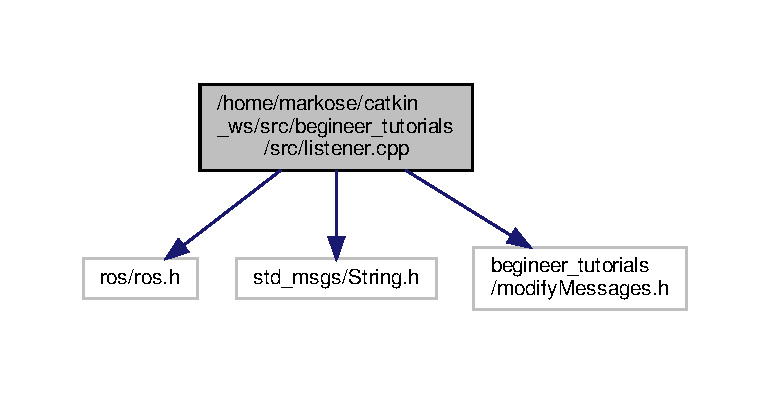
\includegraphics[width=350pt]{listener_8cpp__incl}
\end{center}
\end{figure}
\subsection*{Functions}
\begin{DoxyCompactItemize}
\item 
void \hyperlink{listener_8cpp_ae5c0c11b4a60030ee8df1a3ae0b6f758}{chatter\+Callback} (const std\+\_\+msgs\+::\+String\+::\+Const\+Ptr \&msg)
\begin{DoxyCompactList}\small\item\em This is the interrupt handler. \end{DoxyCompactList}\item 
int \hyperlink{listener_8cpp_a3c04138a5bfe5d72780bb7e82a18e627}{main} (int argc, char $\ast$$\ast$argv)
\end{DoxyCompactItemize}


\subsection{Detailed Description}
Subscriber for beginner tutorials  M\+IT License 2021 Markose Jacob. 



\subsection{Function Documentation}
\mbox{\Hypertarget{listener_8cpp_ae5c0c11b4a60030ee8df1a3ae0b6f758}\label{listener_8cpp_ae5c0c11b4a60030ee8df1a3ae0b6f758}} 
\index{listener.\+cpp@{listener.\+cpp}!chatter\+Callback@{chatter\+Callback}}
\index{chatter\+Callback@{chatter\+Callback}!listener.\+cpp@{listener.\+cpp}}
\subsubsection{\texorpdfstring{chatter\+Callback()}{chatterCallback()}}
{\footnotesize\ttfamily void chatter\+Callback (\begin{DoxyParamCaption}\item[{const std\+\_\+msgs\+::\+String\+::\+Const\+Ptr \&}]{msg }\end{DoxyParamCaption})}



This is the interrupt handler. 


\begin{DoxyParams}{Parameters}
{\em String} & message that arises at the interrupt \\
\hline
\end{DoxyParams}
\begin{DoxyReturn}{Returns}
None 
\end{DoxyReturn}
Here is the caller graph for this function\+:
\nopagebreak
\begin{figure}[H]
\begin{center}
\leavevmode
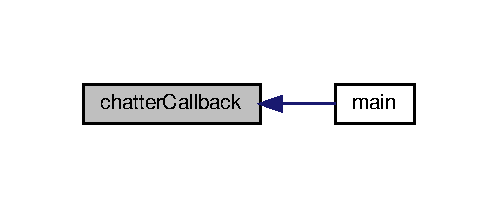
\includegraphics[width=239pt]{listener_8cpp_ae5c0c11b4a60030ee8df1a3ae0b6f758_icgraph}
\end{center}
\end{figure}
\mbox{\Hypertarget{listener_8cpp_a3c04138a5bfe5d72780bb7e82a18e627}\label{listener_8cpp_a3c04138a5bfe5d72780bb7e82a18e627}} 
\index{listener.\+cpp@{listener.\+cpp}!main@{main}}
\index{main@{main}!listener.\+cpp@{listener.\+cpp}}
\subsubsection{\texorpdfstring{main()}{main()}}
{\footnotesize\ttfamily int main (\begin{DoxyParamCaption}\item[{int}]{argc,  }\item[{char $\ast$$\ast$}]{argv }\end{DoxyParamCaption})}

The ros\+::init() function needs to see argc and argv so that it can perform any R\+OS arguments and name remapping that were provided at the command line. For programmatic remappings you can use a different version of init() which takes remappings directly, but for most command-\/line programs, passing argc and argv is the easiest way to do it. The third argument to init() is the name of the node.

You must call one of the versions of ros\+::init() before using any other part of the R\+OS system.

Node\+Handle is the main access point to communications with the R\+OS system. The first Node\+Handle constructed will fully initialize this node, and the last Node\+Handle destructed will close down the node.

The subscribe() call is how you tell R\+OS that you want to receive messages on a given topic. This invokes a call to the R\+OS master node, which keeps a registry of who is publishing and who is subscribing. Messages are passed to a callback function, here called chatter\+Callback. subscribe() returns a Subscriber object that you must hold on to until you want to unsubscribe. When all copies of the Subscriber object go out of scope, this callback will automatically be unsubscribed from this topic.

The second parameter to the subscribe() function is the size of the message queue. If messages are arriving faster than they are being processed, this is the number of messages that will be buffered up before beginning to throw away the oldest ones.

ros\+::spin() will enter a loop, pumping callbacks. With this version, all callbacks will be called from within this thread (the main one). ros\+::spin() will exit when Ctrl-\/C is pressed, or the node is shutdown by the master.Here is the call graph for this function\+:
\nopagebreak
\begin{figure}[H]
\begin{center}
\leavevmode
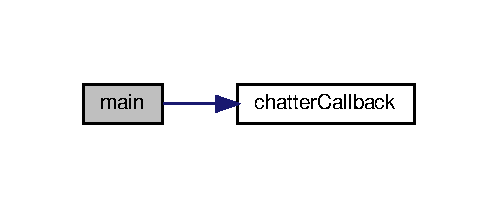
\includegraphics[width=239pt]{listener_8cpp_a3c04138a5bfe5d72780bb7e82a18e627_cgraph}
\end{center}
\end{figure}

\hypertarget{talker_8cpp}{}\section{/home/markose/catkin\+\_\+ws/src/begineer\+\_\+tutorials/src/talker.cpp File Reference}
\label{talker_8cpp}\index{/home/markose/catkin\+\_\+ws/src/begineer\+\_\+tutorials/src/talker.\+cpp@{/home/markose/catkin\+\_\+ws/src/begineer\+\_\+tutorials/src/talker.\+cpp}}


Publisher file  M\+IT License 2021 Markose Jacob.  


{\ttfamily \#include \char`\"{}sstream\char`\"{}}\newline
{\ttfamily \#include \char`\"{}ros/ros.\+h\char`\"{}}\newline
{\ttfamily \#include \char`\"{}std\+\_\+msgs/\+String.\+h\char`\"{}}\newline
{\ttfamily \#include \char`\"{}begineer\+\_\+tutorials/modify\+Messages.\+h\char`\"{}}\newline
Include dependency graph for talker.\+cpp\+:
\nopagebreak
\begin{figure}[H]
\begin{center}
\leavevmode
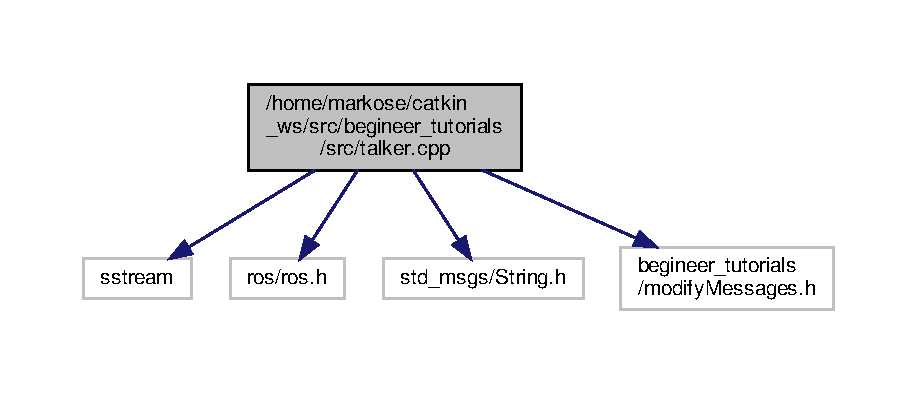
\includegraphics[width=350pt]{talker_8cpp__incl}
\end{center}
\end{figure}
\subsection*{Functions}
\begin{DoxyCompactItemize}
\item 
bool \hyperlink{talker_8cpp_a28aada96921b8dd2f71bcc4a77320cec}{modify\+My\+Message} (begineer\+\_\+tutorials\+::modify\+Messages\+::\+Request \&req, const begineer\+\_\+tutorials\+::modify\+Messages\+::\+Response \&res)
\begin{DoxyCompactList}\small\item\em Ros service server to change ros message being published. \end{DoxyCompactList}\item 
int \hyperlink{talker_8cpp_a3c04138a5bfe5d72780bb7e82a18e627}{main} (int argc, char $\ast$$\ast$argv)
\begin{DoxyCompactList}\small\item\em This tutorial demonstrates simple sending of messages over the R\+OS system. \end{DoxyCompactList}\end{DoxyCompactItemize}
\subsection*{Variables}
\begin{DoxyCompactItemize}
\item 
std\+::string \hyperlink{talker_8cpp_a200c9070506e9fc04c213d1025f9d6fb}{pub\+Message}
\end{DoxyCompactItemize}


\subsection{Detailed Description}
Publisher file  M\+IT License 2021 Markose Jacob. 



\subsection{Function Documentation}
\mbox{\Hypertarget{talker_8cpp_a3c04138a5bfe5d72780bb7e82a18e627}\label{talker_8cpp_a3c04138a5bfe5d72780bb7e82a18e627}} 
\index{talker.\+cpp@{talker.\+cpp}!main@{main}}
\index{main@{main}!talker.\+cpp@{talker.\+cpp}}
\subsubsection{\texorpdfstring{main()}{main()}}
{\footnotesize\ttfamily int main (\begin{DoxyParamCaption}\item[{int}]{argc,  }\item[{char $\ast$$\ast$}]{argv }\end{DoxyParamCaption})}



This tutorial demonstrates simple sending of messages over the R\+OS system. 


\begin{DoxyParams}{Parameters}
{\em argc} & argv \\
\hline
\end{DoxyParams}
\begin{DoxyReturn}{Returns}
None 
\end{DoxyReturn}
The ros\+::init() function needs to see argc and argv so that it can perform any R\+OS arguments and name remapping that were provided at the command line. For programmatic remappings you can use a different version of init() which takes remappings directly, but for most command-\/line programs, passing argc and argv is the easiest way to do it. The third argument to init() is the name of the node.

You must call one of the versions of ros\+::init() before using any other part of the R\+OS system.

Node\+Handle is the main access point to communications with the R\+OS system. The first Node\+Handle constructed will fully initialize this node, and the last Node\+Handle destructed will close down the node.

The advertise() function is how you tell R\+OS that you want to publish on a given topic name. This invokes a call to the R\+OS master node, which keeps a registry of who is publishing and who is subscribing. After this advertise() call is made, the master node will notify anyone who is trying to subscribe to this topic name, and they will in turn negotiate a peer-\/to-\/peer connection with this node. advertise() returns a Publisher object which allows you to publish messages on that topic through a call to publish(). Once all copies of the returned Publisher object are destroyed, the topic will be automatically unadvertised.

The second parameter to advertise() is the size of the message queue used for publishing messages. If messages are published more quickly than we can send them, the number here specifies how many messages to buffer up before throwing some away.

A count of how many messages we have sent. This is used to create a unique string for each message.

The publish() function is how you send messages. The parameter is the message object. The type of this object must agree with the type given as a template parameter to the advertise$<$$>$() call, as was done in the constructor above.Here is the call graph for this function\+:
\nopagebreak
\begin{figure}[H]
\begin{center}
\leavevmode
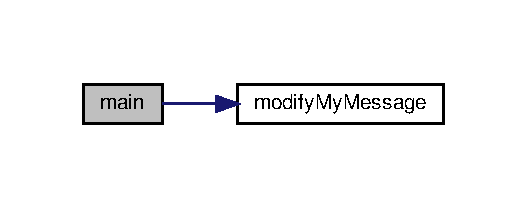
\includegraphics[width=253pt]{talker_8cpp_a3c04138a5bfe5d72780bb7e82a18e627_cgraph}
\end{center}
\end{figure}
\mbox{\Hypertarget{talker_8cpp_a28aada96921b8dd2f71bcc4a77320cec}\label{talker_8cpp_a28aada96921b8dd2f71bcc4a77320cec}} 
\index{talker.\+cpp@{talker.\+cpp}!modify\+My\+Message@{modify\+My\+Message}}
\index{modify\+My\+Message@{modify\+My\+Message}!talker.\+cpp@{talker.\+cpp}}
\subsubsection{\texorpdfstring{modify\+My\+Message()}{modifyMyMessage()}}
{\footnotesize\ttfamily bool modify\+My\+Message (\begin{DoxyParamCaption}\item[{begineer\+\_\+tutorials\+::modify\+Messages\+::\+Request \&}]{req,  }\item[{const begineer\+\_\+tutorials\+::modify\+Messages\+::\+Response \&}]{res }\end{DoxyParamCaption})}



Ros service server to change ros message being published. 


\begin{DoxyParams}{Parameters}
{\em req} & Standard variable of type modify\+Messages\+::\+Request defined in the header file \\
\hline
{\em res} & -\/ Standard variable of type modify\+Messages\+::\+Response defined in the header file \\
\hline
\end{DoxyParams}
\begin{DoxyReturn}{Returns}
bool value 
\end{DoxyReturn}
Here is the caller graph for this function\+:
\nopagebreak
\begin{figure}[H]
\begin{center}
\leavevmode
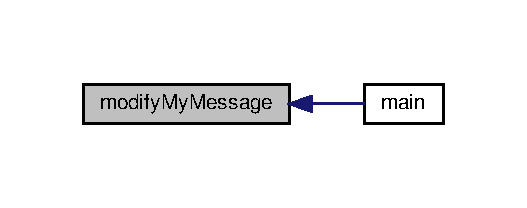
\includegraphics[width=253pt]{talker_8cpp_a28aada96921b8dd2f71bcc4a77320cec_icgraph}
\end{center}
\end{figure}


\subsection{Variable Documentation}
\mbox{\Hypertarget{talker_8cpp_a200c9070506e9fc04c213d1025f9d6fb}\label{talker_8cpp_a200c9070506e9fc04c213d1025f9d6fb}} 
\index{talker.\+cpp@{talker.\+cpp}!pub\+Message@{pub\+Message}}
\index{pub\+Message@{pub\+Message}!talker.\+cpp@{talker.\+cpp}}
\subsubsection{\texorpdfstring{pub\+Message}{pubMessage}}
{\footnotesize\ttfamily std\+::string pub\+Message}

This tutorial demonstrates simple sending of messages over the R\+OS system. 
%--- End generated contents ---

% Index
\backmatter
\newpage
\phantomsection
\clearemptydoublepage
\addcontentsline{toc}{chapter}{Index}
\printindex

\end{document}
